\AtUpperLeft{\raisebox{-1cm}{\textsf{\small \today}}}

\section{Analisi Armonica}
I segnali visti finora sono stati presentati come funzioni descritte da un'espressione analitica; alcuni studiosi, tra cui Fourier,
si accorsero che tali funzioni potevano essere scomposte in somme di altre funzioni (in particolare di fasori, seni e coseni), ossia
è possibile vedere un segnale come \textbf{combinazione lineare} di segnali elementari. Uno strumento che permette di trasformare
un segnale in una combinazione lineare di segnali elementari è lo \textbf{sviluppo in serie di Fourier}.

\subsection{Sviluppo In Serie Di Fourier}
\begin{highlightedeq}
    \paragraph{Teorema.}Data una funzione \textit{periodica} $f(t) : f(t) = f(t + kT)$  $\forall t \in \mathbb{R}, k \in \mathbb{Z}$ e \textit{regolare}
    (ossia che rispetta le condizioni di Dirichlet), allora $f(t)$ piò essere riscritta come una combinazioni lineare di seni e 
    coseni con i propri pesi e le cui frequenze sono multiple di $\frac{1}{T}$ (con $T$ il periodo di $f(t)$).
\end{highlightedeq}

Consideriamo ora i vari multipli:
\begin{itemize}
    \item $n = 0 \longrightarrow f_0 = 0$ è la cosiddetta \textit{componente continua} (un valore costante).
    \item $n = 1 \longrightarrow f_1 = \frac{1}{T}$ viene detta la \textit{frequenza fondamentale}.
    \item $\forall |n| > 1 \longrightarrow f_n = \frac{n}{T}$ viene detta \textit{armonica n-esima}.
\end{itemize}

Gli sviluppi in serie di fourier si presentano in forma \textbf{Trigonometrica} ed \textbf{Esponenziale}

\subsubsection{Forma Esponenziale}
\paragraph{Equazione di Sintesi.}Nella forma esponenziale possiamo esprimere la funzione $f(t)$ come combinazione lineare di fasori \eqref{eq: fasore} $p_n(t)$ a
frequenza $f_n = \frac{1}{T}$ con $T$ il periodo di $f$; è detta \textit{di sintesi} perchè otteniamo $f$ dalla combinazione di fasori
\begin{equation}
    f(t) = \sum_{n = -\infty}^{+\infty} c_n e^{j2\pi \frac{n}{T} t}  \tag{$t \in \mathbb{R}$}
\end{equation}

\paragraph{Equazione di Analisi.} Al contrario della sintesi, noi vogliamo \textit{scomporre} $f$ per ottenere i fasori che la combinano:
\begin{equation}
    c_n = \frac{1}{T} \int_{T} f(t)e^{-j2\pi \frac{n}{T}t} dt \tag{$n \in \mathbb{Z}$}
\end{equation}
Dove $\int_{T}$ è un integrale \textit{di durata T}, ossia che può andare da $0$ a $T$, o da $-T/2$ a $T/2$

\subsubsection{Forma Trigonometrica}
Anche se storicamente è stato al contrario, possiamo derivare a partire dalla forma esponenziale, la forma trigonometrica dello sviluppo.
\paragraph{I Equazione di Sintesi}\begin{equation*}
    f(t) = \sum_{n = -\infty}^{+\infty} c_n e^{j2\pi \frac{n}{T} t} = c_0 + \sum_{n = -\infty}^{+\infty}[ c_n e^{j2\pi \frac{n}{T} t} + c_{-n} e^{-j2\pi \frac{n}{T} t}] \tag{separo i $c_n$}
\end{equation*}
Consideriamo ora $c_{-n}$
\begin{align*}
    c_{-n} =& \frac{1}{T} \int_{T} f(t)e^{-j2\pi \frac{n}{T}t} dt = \\
    =& \frac{1}{T} \int_{T} f(t)\overline{e^{j2\pi \frac{n}{T}t}} dt = \overline{c_n}
\end{align*}
Possiamo vedere il complesso $-j$ come il coniugato del complesso di partenza, dunque:
\begin{align*}
    f(t) =& c_0 + \sum_{n = -\infty}^{+\infty}[ c_n e^{j2\pi \frac{n}{T} t} + \overline{c_{n}} e^{-j2\pi \frac{n}{T}t }] =\\
         =& c_0 + \sum_{n = -\infty}^{+\infty}[ c_n e^{j2\pi \frac{n}{T} t} + \overline{c_{n} e^{j2\pi \frac{n}{T}t} }] = \\
         =& c_o + \sum_{n = -\infty}^{+\infty} 2\mathbb{R}e [c_n e^{j2\pi \frac{n}{T}t}] \tag{proprietà \ref{prop: coniugato}}
\end{align*}
Possiamo dunque notare che, a partire dalla scomposizione di una funzione reale in fasori (complessi) otteniamo ancora qualcosa di completamente reale.
Poniamo ora $c_n = \rho_n e^j \theta_n$, ossia in forma polare:
\begin{align*}
    f(t) &= c_o + \sum_{n = -\infty}^{+\infty} 2\mathbb{R}e [\rho_n e^{j \theta_n} e^{j2\pi \frac{n}{T}t}] =\\
         &= c_o + \sum_{n = -\infty}^{+\infty} 2\mathbb{R}e [\rho_n e^{j2\pi \frac{n}{T}t +\theta_n }] =
\end{align*}
Dal momento che $\mathbb{R}e[e^{j\theta}] = \cos(\theta)$ allora:
\begin{equation}
    f(t) = c_0 + 2 \int_{n = 1}^{+\infty} \rho_n \cos\left(2\pi \frac{n}{T}t +\theta_n\right)
\end{equation}

\paragraph{II Equazione di Sintesi.} Ora poniamo $c_n = a_n - jb_n$:
\begin{align*}
    f(t) =& c_o + \sum_{n = -\infty}^{+\infty} 2\mathbb{R}e \left[c_n e^{j2\pi \frac{n}{T}t}\right] =\\
         =& c_o + \sum_{n = -\infty}^{+\infty} 2\mathbb{R}e \left[(a_n - jb_n) e^{j2\pi \frac{n}{T}t}\right] =\\
         =& c_o + \sum_{n = -\infty}^{+\infty} 2\mathbb{R}e \left[a_n e^{j2\pi \frac{n}{T}t} - jb_n e^{j2\pi \frac{n}{T}t}\right] =\\
\end{align*}
Riscriviamo ora $j$ come $j = e^{j \frac{\pi}{2}}$:
\begin{equation*}
    f(t) = c_o + \sum_{n = -\infty}^{+\infty} 2\mathbb{R}e \left[a_n e^{j2\pi \frac{n}{T}t} - b_n e^{j2\pi \frac{n}{T}t + \frac{\pi}{2}}\right] =
\end{equation*}
Sapendo che, ancora una volta, $\mathbb{R}e[e^{j\theta}] = \cos(\theta)$ allora:
\begin{equation*}
    = c_o + 2\sum_{n = -\infty}^{+\infty} \left[a_n \cos\left(2\pi \frac{n}{T}t\right) - b_n \cos\left(2\pi \frac{n}{T}t + \frac{\pi}{2}\right)\right] =
\end{equation*}
Dal momento che $\cos\left(\theta + \frac{\pi}{2}\right) = -\sin(\theta)$ allora:
\begin{equation}
    f(t) = c_o + 2\sum_{n = -\infty}^{+\infty} \left[a_n \cos\left(2\pi \frac{n}{T}t\right) + b_n \sin\left(2\pi \frac{n}{T}t\right)\right]
\end{equation}
Cerchiamo, a questo punto, di derivare $a_n, b_n$ a partire da $c_n$:
\begin{align*}
    a_n &= \mathbb{R}e[c_n] = \mathbb{R}e\left[ \frac{1}{T} \int_{T} f(t) e^{-j2\pi \frac{n}{T} t} dt \right] =\\
        &= \frac{1}{T} \int_{T} f(t) \mathbb{R}e\left[e^{-j2\pi \frac{n}{T} t}\right] dt =\\
        &= \frac{1}{T} \int_{T} f(t) \cos\left(2\pi \frac{n}{T}t\right)dt
\end{align*}
\begin{align*}
    b_n &= -\mathbb{I}m[c_n] = -\mathbb{I}m\left[ \frac{1}{T} \int_{T} f(t) e^{-j2\pi \frac{n}{T} t} dt \right] =\\
        &= -\frac{1}{T} \int_{T} f(t) \mathbb{I}m\left[e^{-j2\pi \frac{n}{T} t}\right] dt =\\
        &= -\frac{1}{T} \int_{T} f(t) \sin\left(-2\pi \frac{n}{T}t\right)dt =       
\end{align*}
Per la proprietà antisimmetrica del seno $\sin(-\theta) = -\sin(\theta)$ otteniamo:
\begin{equation*}
   b_n = \frac{1}{T} \int_{T} f(t) \sin\left(2\pi \frac{n}{T}t\right)dt 
\end{equation*}

In definitiva, grazie allo sviluppo in serie di Fourier, possiamo trasformare una funzione \textbf{continua, periodica} e regolare in una
somma \textbf{discreta} di fasori con con pesi $\{c_n\}$ nel periodo $[0, T]$; inoltre, grazie ai coefficienti $c_n$ è possibile
conoscere il contributo (o ampiezza) dell'n-esima armonica nello sviluppo di $f(t)$; proprio per questo motivo i $c_n$ rappresentano
lo \textbf{spettro di $f(t)$}. La funzione $f$ di partenza esiste nel \textbf{dominio del tempo} mentre i $c_n$ nel \textbf{dominio delle frequenze}


Una cosa che possiamo notare è che $c_0$ è il valor medio della funzione ed è il contributo che "solleva" la funzione; questo perchè seni/coseni che definiscono
lo sviluppo hanno valor medio nullo.\\

\paragraph{Esempi.} Vedi sul quaderno lo sviluppo del dente di sega e dell'onda quadra.

\subsection{Trasformata di Fourier}
Finora gli sviluppi in serie riguardano solo funzioni continue e periodiche, mentre tutte le altre funzioni non godono di 
questa proprietà. In realtà Fourier scoprì un modo per analizzare lo spettro di qualsiasi funzione reale:\\
Consideriamo una funzione $f(t)$ \textbf{continua e non periodica} e definiamo la sua versione periodica $f_T(t)$ come:
\begin{equation*}
    f_T(t) = f(t) \tag{$-\frac{T}{2} \leq t \leq \frac{T}{2}$}
\end{equation*}
Tale che $f_T(t) = f_T(t + kT)$ con $k \in \mathbb{Z}$ e $T$ il periodo. Quello che fa $f_T(t)$ è di replicare il comportamento
di $f(t)$ nell'intervallo $[-\frac{T}{2}; \frac{T}{2}]$ per tutto $\mathbb{R}$. Dal momento che $f_T(t)$ è periodica e continua, posso 
applicare lo sviluppo in serie di fourier:
\begin{align*}
    f_T(t) &= \sum_{n = -\infty}^{+\infty} c_n e^{j2 \pi j \frac{n}{T}t} = \\
           &= \sum_{n = -\infty}^{+\infty} c_n e^{j2 \pi j f_n t} \tag{con $f_n = \frac{n}{T}$}
\end{align*}
Dove $c_n$ è:
\begin{equation*}
    c_n = \frac{1}{T} \int_{-\frac{T}{2}}^{\frac{T}{2}} f(t) e^{-j2 \pi f_n t}dt
\end{equation*}
Consideriamo ora $\frac{1}{T} = \Delta f$ ossia il passo unitario con cui incrementano le frequenze delle armoniche:
\begin{equation*}
    c_n = \Delta f \int_{-\frac{T}{2}}^{\frac{T}{2}} f(t) e^{-j2 \pi f_n t}dt
\end{equation*}
Facendo tendere il passo unitario a 0 (o meglio, il periodo all'infinito) la versione periodica $f_T(t)$ sarà sempre più
simile alla funzione di partenza, per cui possiamo dire che:
\begin{equation}
    f(t) = \lim_{T \to +\infty} f_T(t)
\end{equation}
Dunque:
\begin{align*}
    f(t) &= \lim_{T \to +\infty} f_T(t) =\\
         &= \lim_{T \to +\infty} \sum_{n = -\infty}^{+\infty} c_n e^{j2 \pi j f_n t} =\\
         &= \lim_{T \to +\infty} \sum_{n = -\infty}^{+\infty} \left[\int_{-\infty}^{+\infty} f(\tau) e^{-j2 \pi f_n \tau}d\tau\right] e^{j2 \pi j f_n t} \Delta f
\end{align*}
Dobbiamo osservare che:
\begin{itemize}
    \item $\int_{-\infty}^{+\infty} f(\tau) e^{-j2 \pi f_n \tau}d\tau$ è una sorta di \textbf{risposta in frequenza} e viene indicata con $F(f)$ (funzione di trasformazione di f)
    \item al tendere di T all'infinito, $\Delta f$ diventa infinitesima, dunque la somma infinita di termini moltiplicati per un'infinitesimo è proprio un integrale
\end{itemize}
\paragraph{Antitrasformata di Fourier.}Per cui:
\begin{align*}
    f(t) &= \lim_{\Delta f \to 0} \sum_{n = -\infty}^{+\infty} F(f_n) e^{j2 \pi j f_n t} df =\\
         &= \int_{-\infty}^{+\infty} F(f) e^{j2 \pi j f t} df =\\
         &= \mathscr{F}^{-1}\{F(f)\}
\end{align*}
E viene detta \textbf{Formula di Sintesi} o \textbf{Antitrasformata di Fourier}
\paragraph{Trasformata di Fourier.}Mentre $F(f)$, anche detta \textbf{Trasformata di Fourier} o \textbf{Formula di Analisi}, è:
\begin{equation}
    F(f) = \int_{-\infty}^{+\infty} f(t) e^{-j2 \pi f t} dt = \mathscr{F}\{f(t)\}
\end{equation}


\begin{minipage}{\textwidth}
    Possiamo dunque vedere quest'importante relazione:\\
\begin{center}
    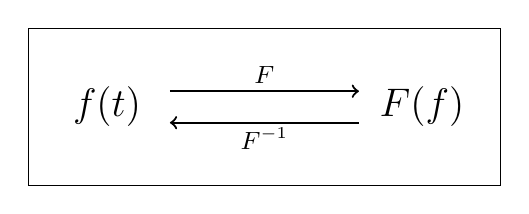
\begin{tikzpicture}
        % Box
        \node[draw, minimum width=6cm, minimum height=2cm] at (0,0) {};
        
        % Left side: Larger Time domain function
        \node at (-2, 0) {\Large $f(t)$};
        
        % Right side: Larger Frequency domain function
        \node at (2, 0) {\Large $F(f)$};
        
        % Fourier transform arrow, closer to center
        \draw[->, thick] (-1.2, 0.2) -- (1.2, 0.2);
        \node at (0, 0.4) {\small $\mathscr{F}$};
        
        % Inverse Fourier transform arrow, closer to center
        \draw[<-, thick] (-1.2, -0.2) -- (1.2, -0.2);
        \node at (0, -0.4) {\small $\mathscr{F}^{-1}$};
    \end{tikzpicture}
    \end{center}
    Con $f : \mathbb{R} \rightarrow \mathbb{C}$ e $F : \mathbb{R} \rightarrow \mathbb{C}$. Sebbene quasi sempre lo spettro di una
funzione f è complesso, quindi tridimensionale, possiamo raccontare \textbf{frequenze} e \textbf{ampiezze} tramite le funzioni:
\begin{itemize}
    \item \textbf{Spettro d'Ampiezza} $|F(f)| : \mathbb{R} \rightarrow \mathbb{R}$
    \item \textbf{Spettro di Fase} $\angle F(f) : \mathbb{R} \rightarrow \mathbb{R}$
\end{itemize} 

\end{minipage}
